\subsection{Link Budget}
\paragraph
\ Astrea constellation main satellite must be able to stablish three different telecommunications link: 
\begin{itemize}
	\item Space to Ground link.
	\item Space to Space link between Astrea satellites.
	\item Space to Space link between client ans Astrea satellites.
\end{itemize} 

\paragraph
\ The link budget calculations are mostly calculated using the following fonts:\cite{linkBudget}.

\subsubsection{Communications Basics}
\paragraph
\
\cite{an9804.pdf}
When evaluating a wireless link, the three most important questions to be answered are:\\
\begin{enumerate}
	\item How much radio frequency (RF) power is available?
	\item How much bandwidth is available?
	\item What is the required reliability (as defined by Bit Error Rate, or BER)?
\end{enumerate}

The upper limit in terms of data rate is given by Shannon's Channel Capacity Theorem:
\begin{equation}
	C=Blog_2(1+S/N)
	\label{channelCapacity}
\end{equation}
where:
\begin{align*}
	C&= \text{channel capacity (bits/s)}\\
	B&= \text{channel bandwidth (Hz)}\\
	S&= \text{signal strength (watts)}\\
	N&= \text{noise power (watts)}
\end{align*}

\paragraph{Transmission Losses}
\ In any satellite transmission, there are always losses from various sources. Some of
those losses may be constant, others are dependent of statistical data and others vary
with the weather conditions, especially with rain.

\subsubsection{Propagation losses}
a
\subsubsubsection{Free Space Losses}
\paragraph{Range and Path Loss}
\
Another key consideration is the issue of range. As radio
waves propagate in free space, power falls off as the square
of range. For a doubling of range, power reaching a receiver
antenna is reduced by a factor of four. This effect is due to
the spreading of the radio waves as they propagate, and can
be calculated by:
\begin{equation}
L=20log_{10}(4\pi D/\lambda)
\label{FSP}
\end{equation}
where:
\begin{align*}
	D&= \text{the distance between receiver and transmitter}\\
	\lambda&= \text{free space wavelength = c/f}\\
	c&= \text{speed of light}(3\mathrm{x}10^8m/s)\\
	f&= \text{frequency (Hz)}
\end{align*}
a
\subsubsubsection{Atmospheric Losses}
\paragraph{Ionospheric Effects}
\paragraph{Tropospheric Effects}
\paragraph{Local Effects}
\subsubsubsection{Pointing Losses}
\subsubsubsection{Multipath and Fade Margin}
\paragraph
\
Multipath occurs when waves emitted by the transmitter
travel along a different path and interfere destructively with
waves travelling on a direct line-of-sight path. This is
sometimes referred to as signal fading. This phenomenon
occurs because waves travelling along different paths may
be completely out of phase when they reach the antenna,
thereby cancelling each other.\\

The amount of extra RF power radiated to overcome this
phenomenon is referred to as fade margin. The exact
amount of fade margin required depends on the desired
reliability of the link, but a good rule-of-thumb is 20dB to
30dB.


\subsubsection{Local Losses}
\subsubsubsection{Equipament Losses}
\subsubsubsection{Environment Losses}

\subsubsection{Modulation Technique}
\paragraph
\ Modulation technique is a key consideration. This is the
method by which the analogue or digital information is
converted to signals at RF frequencies suitable for
transmission. Selection of modulation method determines
system bandwidth, power efficiency, sensitivity, and
complexity. Most of us are familiar with Amplitude
Modulation (AM) and Frequency Modulation (FM) because
of their widespread use in commercial radio. Phase
Modulation is another important technique. It is used in
applications such as Global Position System (GPS)
receivers and some cellular telephone networks. \cite{bibid}\\

For the purposes of link budget analysis, the most important
aspect of a given modulation technique is the Signal-to-
Noise Ratio (SNR) necessary for a receiver to achieve a
specified level of reliability in terms of BER.\\

\begin{figure}[h]
	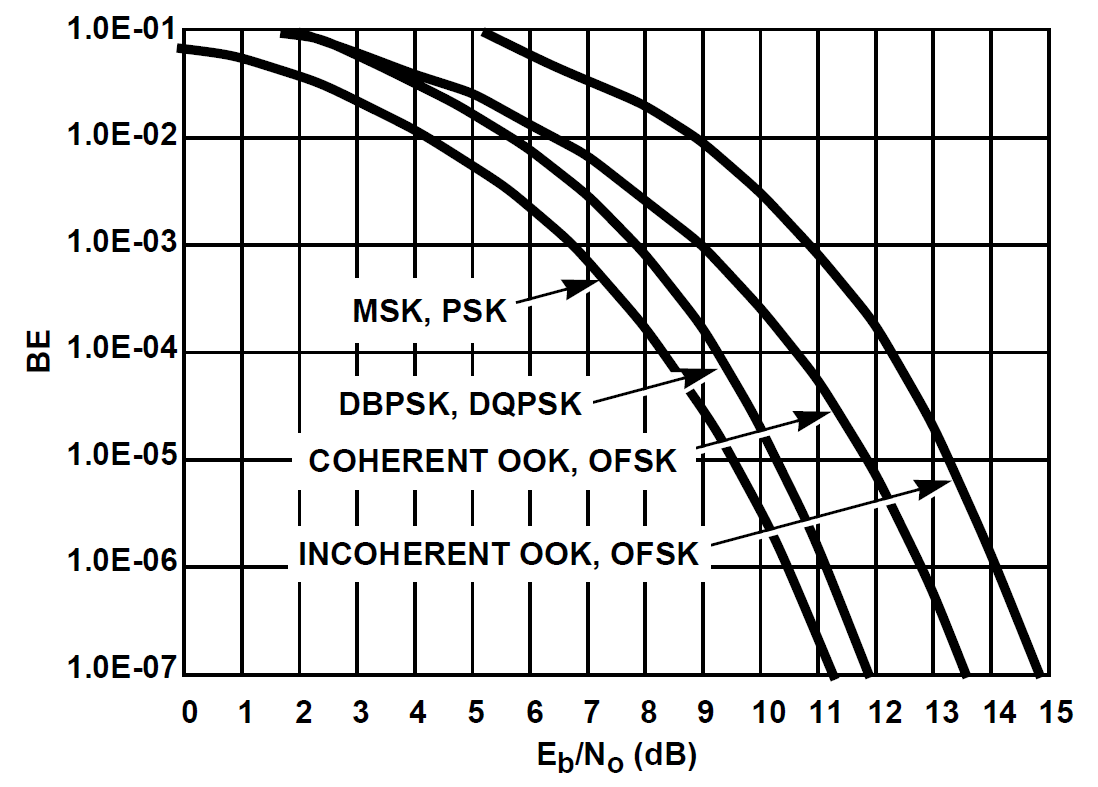
\includegraphics[scale=0.3]{./sections/SatelliteDesign/images/BEvsSNR}
	\centering
	\caption{Probability of bit error for common modulation methods\cite{cubesatdimensions}}
	\label{BEvsSNR}
\end{figure}
A graph of Eb/No
vs BER is shown in Figure \ref{BEvsSNR}. $E_b/N_o$ is a measure of the
required energy per bit relative to the noise power. Note that
$E_b/N_o$ is independent of the system data rate. In order to
convert from $E_b/N_o$ to $SNR$, the data rate and system
bandwidth must be taken into account as shown below:
\begin{equation}
SNR=(E_b/N_o)(R/B_T)
\label{SNReq}
\end{equation}
where:
\begin{align*}
	E_b&= \text{Energy required per bit of information}\\
	N_o&= \text{thermal noise in 1Hz of bandwidth}\\
	R&= \text{system data rate}\\
	B_T&= \text{system bandwidth}
\end{align*}


\subsubsection{System Noise}
\paragraph{Channel Noise}
\
All objects which have heat emit RF energy in the form of random (Gaussian) noise. The amount of radiation emitted can be calculated by \cite{linkBudget}:
\begin{equation}
N=kTB
\label{noise}
\end{equation}
where:
\begin{align*}
	N&= \text{noise power (watts)}\\
	k&= \text{Boltzman's constant}(1.38\mathrm{x}10^{-23}J/K)\\
	T&= \text{system temperature, usually assumed to be 290K}\\
	B&= \text{channel bandwidth (Hz)}
\end{align*}

This is the lowest possible noise level for a system with a given physical temperature. For most applications, temperature is typically assumed to be room temperature (290K). Equations \ref{channelCapacity} and \ref{noise} demonstrate that RF power and bandwidth can be traded off to achieve a given performance level (as defined by BER).

\subsubsection{Link Budget Calculation}
\paragraph{Methodology} \ From the expected requirements fixed on the Project Charter, general radio systems parameters will computed, in order to have a reference to look for the best communications system on board the Astrea satellites.

$EIRP=P_T-L_T-G_T$
